\documentclass[12pt,a4paper]{article}
\usepackage[utf8]{inputenc}
\usepackage[spanish]{babel}
\usepackage{float}
\usepackage{amsmath}
\usepackage{amsfonts}
\usepackage{subcaption}
\usepackage{amssymb}
\usepackage{graphicx}
\usepackage{hyperref}
\usepackage{braket} % Paquete ideal para la notación de Dirac
\graphicspath{{Pics/}}
\title{Sobre las caminatas en 4D.}
\author{Saúl Nájera Allara}
\date{}
\begin{document}
\maketitle
Sea $\mathcal{H}_p$ el espacio de Hilbert de la posición y $\mathcal{H}_c$ el espacio de Hilbert de la moneda. El estado del caminante 
pertenece al espacio:
\begin{equation*}
\mathcal{H}=\mathcal{H}_p \otimes \mathcal{H}_c
\end{equation*}
Para una caminata cuántica en dos dimensiones, podemos interpretar al estado de la moneda como:
\begin{enumerate}
    \item Un qudit, un espacio de Hilbert de cuatro dimensiones.
    \item Un sistema compuesto de dos qubits, donde uno se encarga de la elección del movimiento horizontal y otro del movimiento vertical.
\end{enumerate}
\section{La caminata si la moneda es un Qudit.}
Considerando que $dim\, \mathcal{H}_c=4$ y sea $\{c_i\}_{i=1,\cdots,4}$ una base ortonormal de $\mathcal{H}_c$.
Podemos interpretar que $\ket{c_1}$ denota la dirección izquierda, $\ket{c_2}$ arriba, $\ket{c_3}$ derecha, $\ket{c_4}$ abajo.

Dado $\ket{c}\in \mathcal{H}_c$, se sigue que:
\begin{equation*}
    \ket{c}=\sum_{m=1}^{4}\lambda_m \ket{c_m}.
\end{equation*}
Pidiendo que $\bra{c}\ket{c}=1$, se obtiene:
\begin{equation*}
    \sum_{m=1}^{4}|\lambda_n|^2=1.
\end{equation*}
Un estado localizado genérico es de la forma:
\begin{equation}
    \ket{\psi}=\sum_{m=1}^{4}\ket{x,y}\otimes\ket{\lambda_m c_m}.
    \label{eq:eq1}
\end{equation}
Si $\Omega$ denota el interior del estadio, entonces se define la acción del operador shift condicional S sobre un estado de la forma dada en \eqref{eq:eq1} como:
\begin{equation}
   S\ket{x,y}\otimes \ket{c_m}=
   \begin{cases}
        \ket{x+\delta_m^{(x)},y+\delta_m^{(y)}}\otimes \ket{c_m} & \text{si $(x,y)\in \Omega$}.
        \\
        \ket{x,y}\otimes \ket{\bar{c}_m} & \text{si $(x,y)\notin \Omega$}.
    \end{cases}
\end{equation}
Donde $\delta_m^{(x)}$, $\delta_m^{(x)}$, denotan desplazamientos unitarios (se desplazan a alguno de los vértices más cercanos) que depende de una regla fija asociada los $c_m$
y $\bar{c_m}$ denota invertir la dirección de $c_m$, es decir, izquierda pasa a derecha, arriba pasa a abajo, etc.
En particular, se considera la regla de asignación según:
\begin{equation*}
\begin{cases}
    \text{Si $\ket{c_m}=\ket{c_1}$} & \text{, entonces }\delta_1^{(x)}=-1\,,\delta_1^{(y)}=0. \\
     \text{Si $\ket{c_m}=\ket{c_2}$} & \text{, entonces }\delta_2^{(x)}=0\,,\delta_2^{(y)}=1. \\
      \text{Si $\ket{c_m}=\ket{c_3}$} & \text{, entonces }\delta_3^{(x)}=1\,,\delta_3^{(y)}=0. \\
       \text{Si $\ket{c_m}=\ket{c_4}$} & \text{, entonces }\delta_4^{(x)}=0\,,\delta_4^{(y)}=-1. \\
\end{cases}
\end{equation*}
Defínase el operador moneda según:
\begin{equation}
   C(\theta)= 1_p\otimes M(\theta)
\end{equation}
Donde $M(\theta)$ es una matriz de dimensión $4\times 4$ unitaria.
Un ejemplo de matriz $M(\theta)$ es la matriz de Grover, dada según
\begin{equation*}
M(\theta) = 
\begin{pmatrix}
-\sin^2\theta & \cos^2\theta & \cos\theta\sin\theta & \cos\theta\sin\theta \\
\cos^2\theta & -\sin^2\theta & \cos\theta\sin\theta & \cos\theta\sin\theta \\
\cos\theta\sin\theta & \cos\theta\sin\theta & -\cos^2\theta & \sin^2\theta \\
\cos\theta\sin\theta & \cos\theta\sin\theta & \sin^2\theta & -\cos^2\theta
\end{pmatrix}
\end{equation*}
En particular, para $\theta=\frac{\pi}{4}$, se tiene:
\begin{equation*}
M(\frac{\pi}{4}) = 
\begin{pmatrix}
-1/2 & 1/2 & 1/2 & 1/2 \\
1/2 & -1/2 & 1/2 & 1/2 \\
1/2 & 1/2 & -1/2 & 1/2 \\
1/2 & 1/2 & 1/2 & -1/2
\end{pmatrix}
\end{equation*}
$M(\frac{\pi}{4})$ es unitaria.

Si consideramos que los $\ket{c_i}$ son los vectores canónicos $\ket{e_i}$, entonces se tiene para $\theta=\frac{\pi}{4}$ que:
\begin{align*}
\begin{cases}
M(\frac{\pi}{4})\ket{c_1}=-\frac{1}{2}\ket{c_1}+\frac{1}{2}\ket{c_2}+\frac{1}{2}\ket{c_3}+\frac{1}{2}\ket{c_4}
\\
M(\frac{\pi}{4})\ket{c_2}=\frac{1}{2}\ket{c_1}-\frac{1}{2}\ket{c_2}+\frac{1}{2}\ket{c_3}+\frac{1}{2}\ket{c_4}
\\
M(\frac{\pi}{4})\ket{c_3}=\frac{1}{2}\ket{c_1}+\frac{1}{2}\ket{c_2}-\frac{1}{2}\ket{c_3}+\frac{1}{2}\ket{c_4}
\\
M(\frac{\pi}{4})\ket{c_4}=\frac{1}{2}\ket{c_1}+\frac{1}{2}\ket{c_2}+\frac{1}{2}\ket{c_3}-\frac{1}{2}\ket{c_4}
\end{cases}
\end{align*}
Vemos que
\begin{equation*}
M(\theta)\ket{c_i}=\sum_{k=1}^{4}\alpha_k \ket{c_k}\, , \alpha_k \neq 0
\end{equation*}
Note que al ser unitaria, se preserva la norma y por tanto $\alpha_i$ son amplitudes de probabilidad.
El operador evolución se define según:
\begin{equation}
U=S\cdot C(\theta).
\end{equation}
Consideremos el primer paso de un caminante de la forma:
\begin{equation}
    \ket{\psi_0}=\ket{x,y}\otimes\ket{c_1}
    \label{eq:firststate}
\end{equation}
Entonces:
\begin{align*}
\ket{\psi_1}= S\cdot C(\theta)\ket{\psi_0}=S\cdot C(\theta)\ket{x,y}\otimes\ket{c_1}
\\
=S\ket{x,y}\otimes M(\theta)\ket{c_1}
\\
=S\ket{x,y}\otimes \sum_{k=1}^{4}\alpha_k \ket{c_k}
\\
\ket{\psi_1}=\sum_{k=1}^{4}S\ket{x,y}\otimes \alpha_k \ket{c_k}
\end{align*}
Aplicando las reglas de asignación establecidas, se tendría que:
\begin{equation}
    \ket{\psi_1}=\ket{x-1,y}\otimes \alpha_1 \ket{c_1}+\ket{x,y+1}\otimes \alpha_2 \ket{c_2}+\ket{x+1,y}\otimes \alpha_3 \ket{c_3}
    +\ket{x,y-1}\otimes \alpha_4 \ket{c_4}
    \label{eq:firststep}
\end{equation}
Inmediantamente podemos concluir que la evolución a un primer paso de cualquier estado localizado de la forma \eqref{eq:eq1} se obtienen cuatro estados localizados en las casillas inmediatas a la posición inicial
y para cada estado se tiene como estado de moneda la dirección en la que se movió con un peso $\alpha_k$ de que suceda.
Las $\alpha_i$ dependen directamente de $M(\theta)$ y para el caso de $\theta=\frac{\pi}{4}$ se para cada dirección posible, igual probabilidad.

Para estados de la forma 
\begin{equation}
    \ket{\phi}=\ket{x,y}\otimes \lambda \ket{c_i}
\end{equation}
Considere 
\begin{equation*}
    \ket{\phi}=(1_p\otimes \lambda)\ket{x,y}\otimes \ket{c_i}
\end{equation*}
Y se verifica que: \[[U,1_p\otimes \lambda]=0\]
Y aplicando el mismo análisis que antes, se sigue que, para el estado
\[\ket{\phi_0}=\ket{x,y}\otimes \lambda \ket{c_1}\]
Se tiene la evolución
\begin{align*}
   \ket{\phi_1}= U\ket{\phi_0}=(1_p\otimes \lambda )U\ket{x,y}\otimes \ket{c_1}
   \\
   \\
  \ket{\phi_1} =(1_p\otimes \lambda )(\ket{x-1,y}\otimes \alpha_1 \ket{c_1}+\ket{x,y+1}\otimes \alpha_2 \ket{c_2}
   \\
   +\ket{x+1,y}\otimes \alpha_3 \ket{c_3}+\ket{x,y-1}\otimes \alpha_4 \ket{c_4})
   \\\\
    \ket{\phi_1} =\ket{x-1,y}\otimes \lambda\alpha_1 \ket{c_1}+\ket{x,y+1}\otimes \lambda\alpha_2 \ket{c_2}
   \\
   +\ket{x+1,y}\otimes \lambda\alpha_3 \ket{c_3}+\ket{x,y-1}\otimes \lambda\alpha_4 \ket{c_4}
\end{align*}

\subsection{Sobre la elección de la moneda, $M(\theta)$}
La ecuación \eqref{eq:firststep} permite ver que la elección de $M(\theta)$ determina los pesos $\alpha_k$ que
dictan las posibles direcciones del caminante de la forma \eqref{eq:firststate} en el siguiente paso.

\begin{itemize}

    \item ¿Toda $M(\theta)$ unitaria es candidata a ser una mondeda?
    \item ¿Que tanto se diferencian las caminatas según la elección del tipo de moneda $M(\theta)$?
    \item ¿Las correspondencias con RMT e integrabilidad son invariantes ante la elección de $M(\theta)$ apropiados?

\end{itemize}
\subsubsection{Moneda de Grover}
Dada según:
\begin{equation}
    M_{Grov}(\theta) = 
\begin{pmatrix}
-\sin^2\theta & \cos^2\theta & \cos\theta\sin\theta & \cos\theta\sin\theta \\
\cos^2\theta & -\sin^2\theta & \cos\theta\sin\theta & \cos\theta\sin\theta \\
\cos\theta\sin\theta & \cos\theta\sin\theta & -\cos^2\theta & \sin^2\theta \\
\cos\theta\sin\theta & \cos\theta\sin\theta & \sin^2\theta & -\cos^2\theta
\end{pmatrix}
    \label{eq:GroverCoin}
\end{equation}
Se estudiaran las eigenfases del operador evolución $U=SM_{Grov}$, determinando su densidad de estados y en base a esto 
el factor de forma espectral y el espaciamiento a primer vecino.

\begin{itemize}

\item \textbf{\large Para un estadio rectangular:}

Considerando un estadio rectangular, con dimensiones $L_x=50$ y $L_y=25$:
\begin{figure}[H]
    \centering
    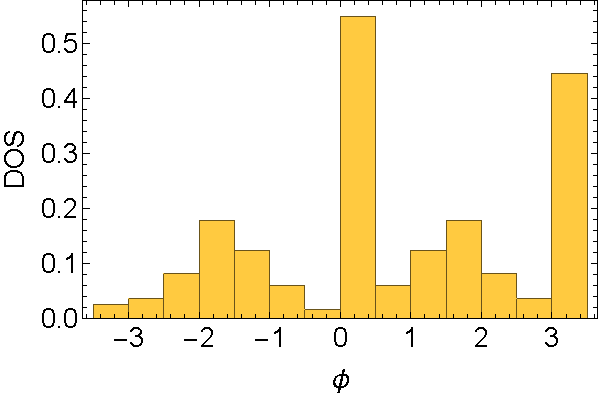
\includegraphics[width=0.8\textwidth]{DoSRectQudit.pdf}
    \caption{DoS de las eigenfases del operador evolución, note los picos centrados alrededor de $0\,\text{y}\,\pi$}
\end{figure}
Luego de remover los picos, se obtiene:
\begin{figure}[H]
    \centering
    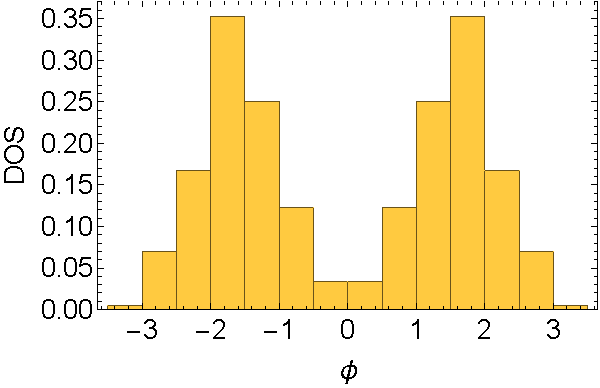
\includegraphics[width=0.8\textwidth]{DoSFilteredRectQudit.pdf}
    \caption{DoS de las eigenfases filtradas del operador evolución, note los picos centrados alrededor de $0\,\text{y}\,\pi$}
\end{figure}
A partir de las eigenfases filtradas se hace la estadística espectral:
\begin{figure}[H]
    \centering
    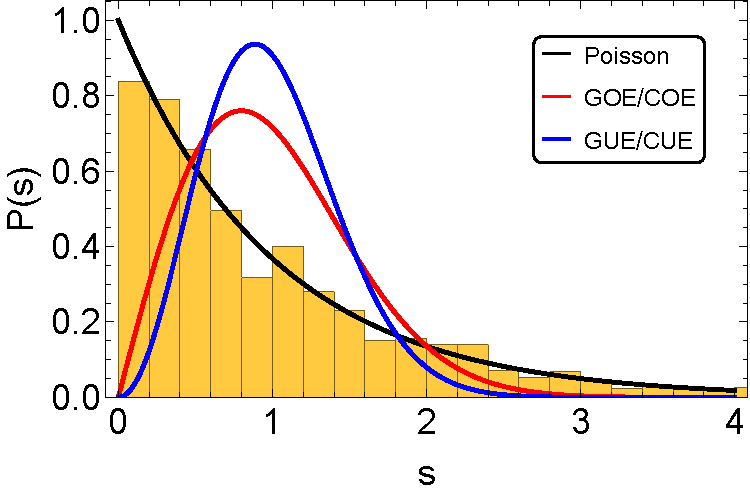
\includegraphics[width=0.8\textwidth]{SpacingRectQudit.pdf}
    \caption{Espaciamiento a primer vecino de las eigenfases filtradas del operador evolución.}
\end{figure}
\begin{figure}[H]
    \centering
    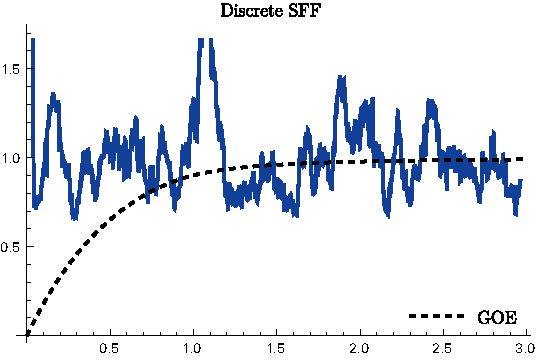
\includegraphics[width=0.8\textwidth]{SFFRectQudit.pdf}
    \caption{Factor de forma espectral de las eigenfases filtradas del operador evolución.}
\end{figure}
\hfill
\item \textbf{\large Para un estadio bunimovich:}

 Empleando ahora un estadio bunimovich, de dimensiones $L=35$ y $R=25$, la DoS fue igualmente filtrada para remover los picos centradados alrededor de $0$ y $\pi$.

A partir de las eigenfases filtradas se hace la estadística espectral:
\begin{figure}[H]
    \centering
    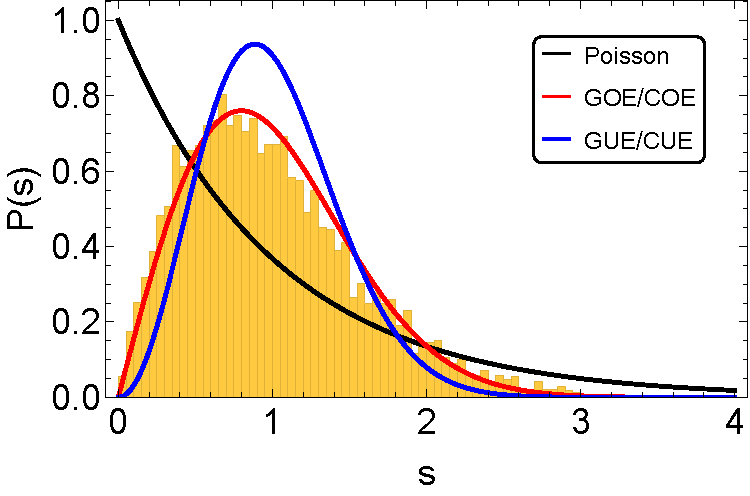
\includegraphics[width=0.8\textwidth]{SpacingBunQudit.pdf}
    \caption{Espaciamiento a primer vecino de las eigenfases filtradas del operador evolución.}
\end{figure}
\begin{figure}[H]
    \centering
    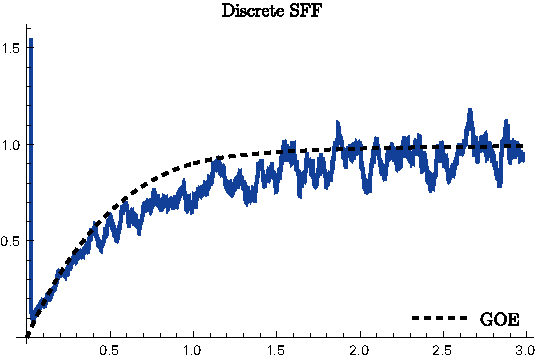
\includegraphics[width=0.8\textwidth]{SFFBunQudit.pdf}
    \caption{Factor de forma espectral de las eigenfases filtradas del operador evolución.}
\end{figure}

\item \textbf{\large Para un estadio elipse:}

 Empleando ahora un estadio elipse, con semi-eje mayor de $A=50$ y semi-eje menor de $B=25$, la DoS fue igualmente filtrada para remover los picos centradados alrededor de $0$ y $\pi$.

A partir de las eigenfases filtradas se hace la estadística espectral:
\begin{figure}[H]
    \centering
    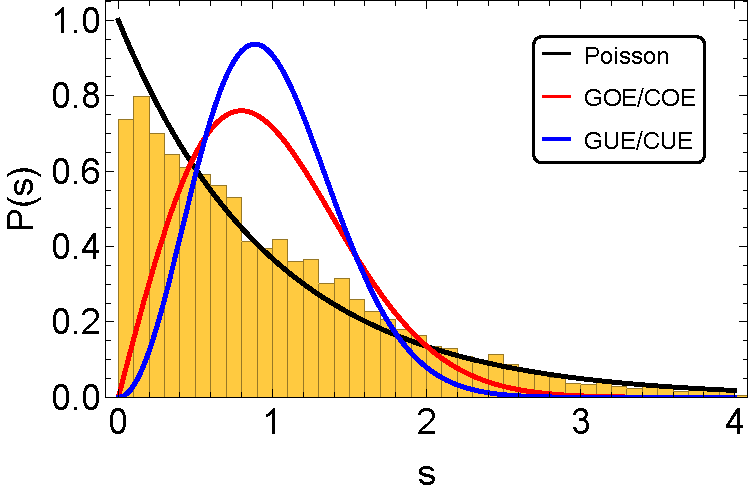
\includegraphics[width=0.8\textwidth]{SpacingElipseQudit.pdf}
    \caption{Espaciamiento a primer vecino de las eigenfases filtradas del operador evolución.}
\end{figure}
\begin{figure}[H]
    \centering
    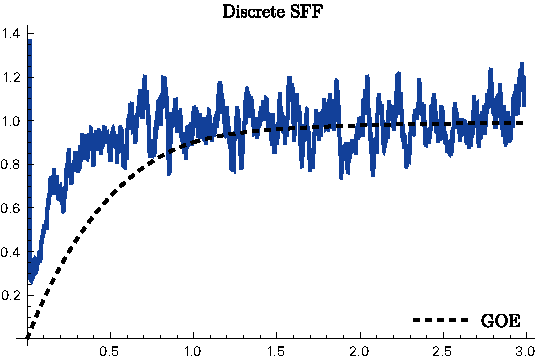
\includegraphics[width=0.8\textwidth]{SFFElipseQudit.pdf}
    \caption{Factor de forma espectral de las eigenfases filtradas del operador evolución.}
\end{figure}

\item \textbf{\large Para un estadio cardioide:}

 Empleando ahora un estadio cardiode, con parámetro de escala $R=17$, siendo $r=2R(1-\cos(\theta))$
 
 la DoS fue igualmente filtrada para remover los picos centradados alrededor de $0$ y $\pi$.

A partir de las eigenfases filtradas se hace la estadística espectral:
\begin{figure}[H]
    \centering
    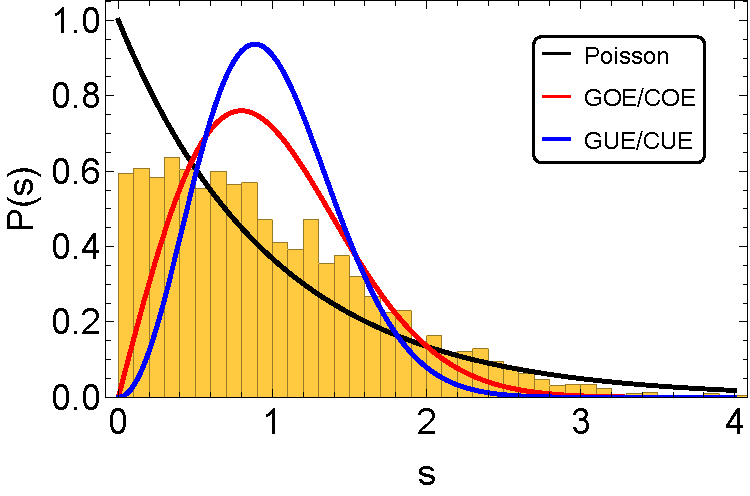
\includegraphics[width=0.8\textwidth]{SpacingCardQudit.pdf}
    \caption{Espaciamiento a primer vecino de las eigenfases filtradas del operador evolución.}
\end{figure}
\begin{figure}[H]
    \centering
    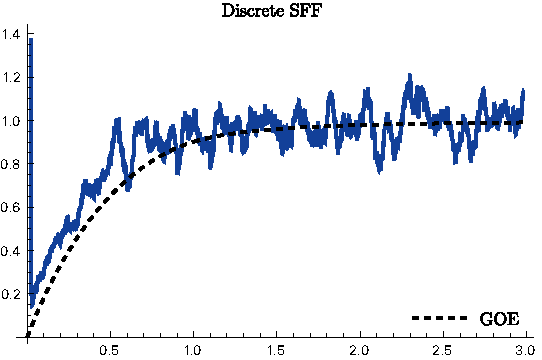
\includegraphics[width=0.8\textwidth]{SFFCardQudit.pdf}
    \caption{Factor de forma espectral de las eigenfases filtradas del operador evolución.}
\end{figure}

\item \textbf{\large Para un estadio 1/8 de sinaí:}

 Empleando ahora un estadio sinaí, con $L=160$ y $R=140$.
 la DoS fue igualmente filtrada para remover los picos centradados alrededor de $0$ y $\pi$.

A partir de las eigenfases filtradas se hace la estadística espectral:
\begin{figure}[H]
    \centering
    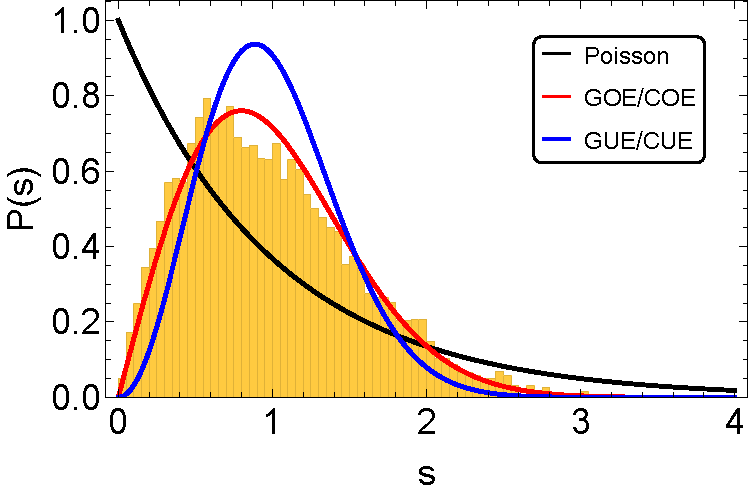
\includegraphics[width=0.8\textwidth]{SpacingSinaiQudit.pdf}
    \caption{Espaciamiento a primer vecino de las eigenfases filtradas del operador evolución.}
\end{figure}
\begin{figure}[H]
    \centering
    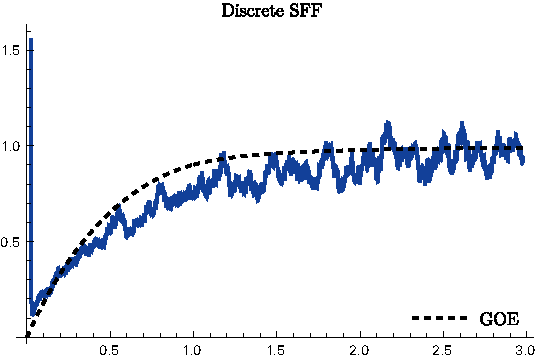
\includegraphics[width=0.8\textwidth]{SFFSinaiQudit.pdf}
    \caption{Factor de forma espectral de las eigenfases filtradas del operador evolución.}
\end{figure}


\end{itemize}

\subsubsection{Moneda de Haadamar}
Dada según
\begin{equation}
    H_2 = \frac{1}{\sqrt{2}}
    \begin{pmatrix}
        1 & 1 \\
        1 & -1
    \end{pmatrix}, 
    \quad
    H_4 = H_2 \otimes H_2 = \frac{1}{2}
    \begin{pmatrix}
        1 &  1 &  1 &  1 \\
        1 & -1 &  1 & -1 \\
        1 &  1 & -1 & -1 \\
        1 & -1 & -1 &  1
    \end{pmatrix}
    \label{eq:Haar}
\end{equation}

\begin{itemize}

\item \textbf{\large Para un estadio rectangular:}

Considerando un estadio rectangular, con dimensiones $L_x=35$ y $L_y=25$:
\begin{figure}[H]
    \centering
    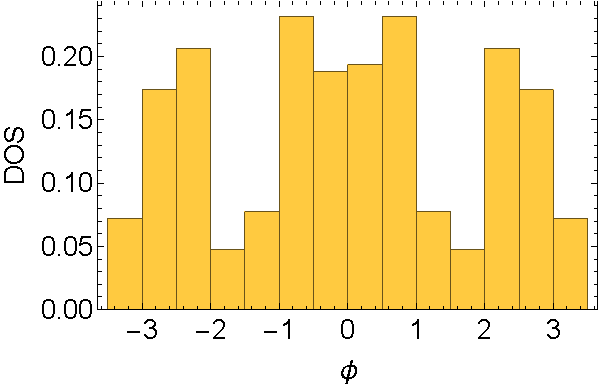
\includegraphics[width=0.8\textwidth]{DoSRectQuditHaad.pdf}
    \caption{DoS de las eigenfases del operador evolución.}
\end{figure}
Para esta moneda no fue necesario emplear un filtrado en las eigenfases.
\begin{figure}[H]
    \centering
    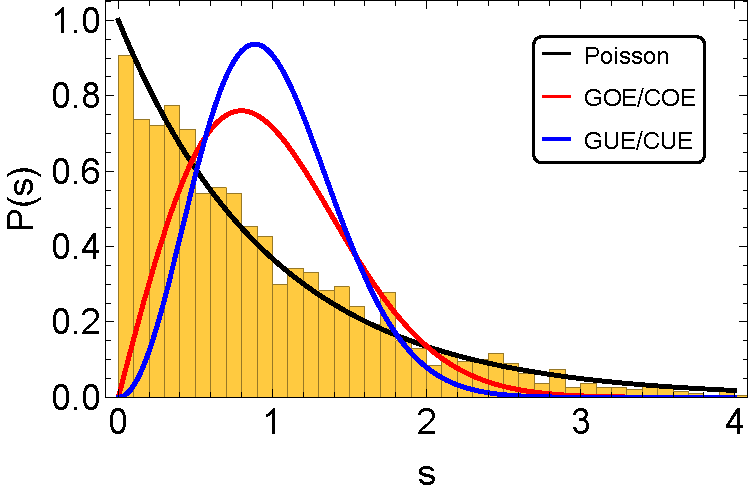
\includegraphics[width=0.8\textwidth]{SpacingRectQuditHaad.pdf}
    \caption{Espaciamiento a primer vecino de las eigenfases del operador evolución.}
\end{figure}
\begin{figure}[H]
    \centering
    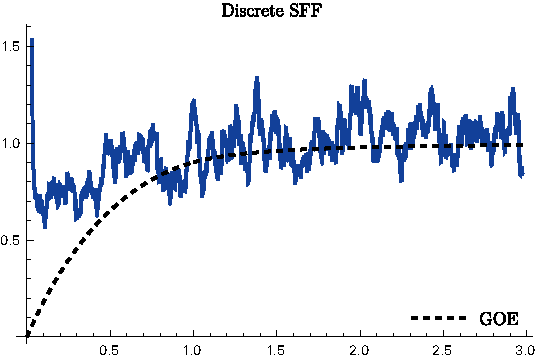
\includegraphics[width=0.8\textwidth]{SFFRectQuditHaad.pdf}
    \caption{Factor de forma espectral de las eigenfases del operador evolución.}
\end{figure}
\hfill
\item \textbf{\large Para un estadio bunimovich:}

 Empleando ahora un estadio bunimovich, de dimensiones $L=30$ y $R=25$.
\begin{figure}[H]
    \centering
    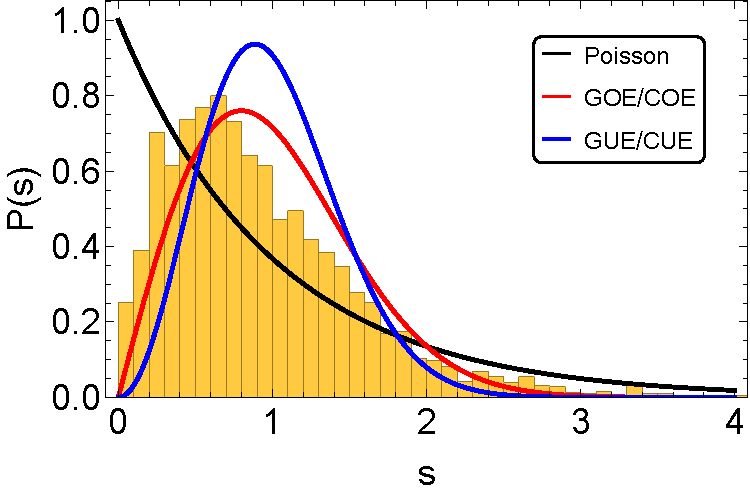
\includegraphics[width=0.8\textwidth]{SpacingBunQuditHaad.pdf}
    \caption{Espaciamiento a primer vecino de las eigenfases del operador evolución.}
\end{figure}
\begin{figure}[H]
    \centering
    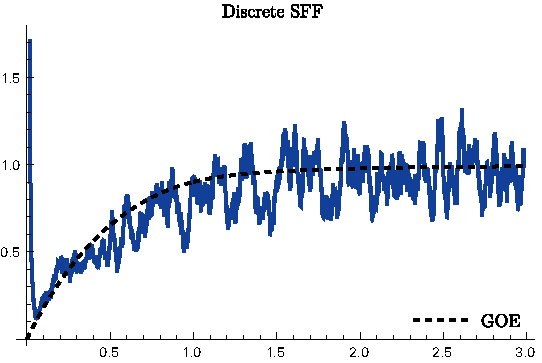
\includegraphics[width=0.8\textwidth]{SFFBunQuditHaad.pdf}
    \caption{Factor de forma espectral de las eigenfases del operador evolución.}
\end{figure}

\item \textbf{\large Para un estadio elipse:}

 Empleando ahora un estadio elipse, con semi-eje mayor de $A=20$ y semi-eje menor de $B=15$.
\begin{figure}[H]
    \centering
    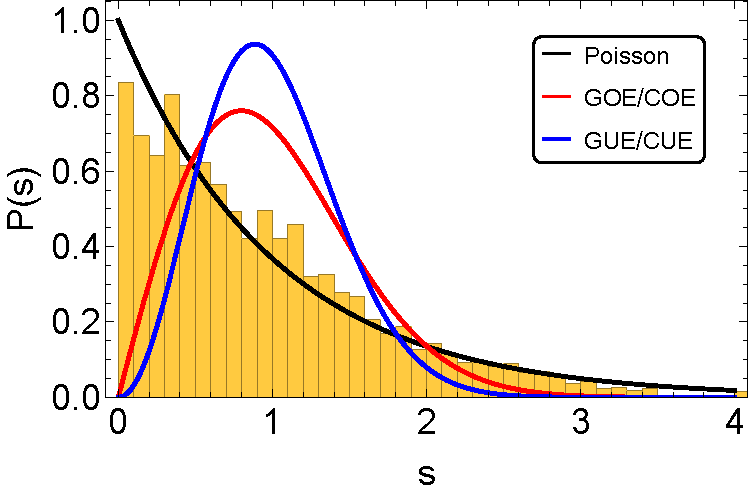
\includegraphics[width=0.8\textwidth]{SpacingElipseQuditHaad.pdf}
    \caption{Espaciamiento a primer vecino de las eigenfases del operador evolución.}
\end{figure}
\begin{figure}[H]
    \centering
    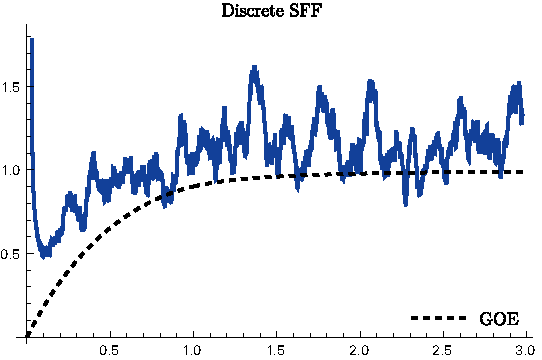
\includegraphics[width=0.8\textwidth]{SFFElipseQuditHaad.pdf}
    \caption{Factor de forma espectral de las eigenfases del operador evolución.}
\end{figure}

\item \textbf{\large Para un estadio cardioide:}

 Empleando ahora un estadio cardiode, con parámetro de escala $R=7$, siendo $r=2R(1-\cos(\theta))$
\begin{figure}[H]
    \centering
    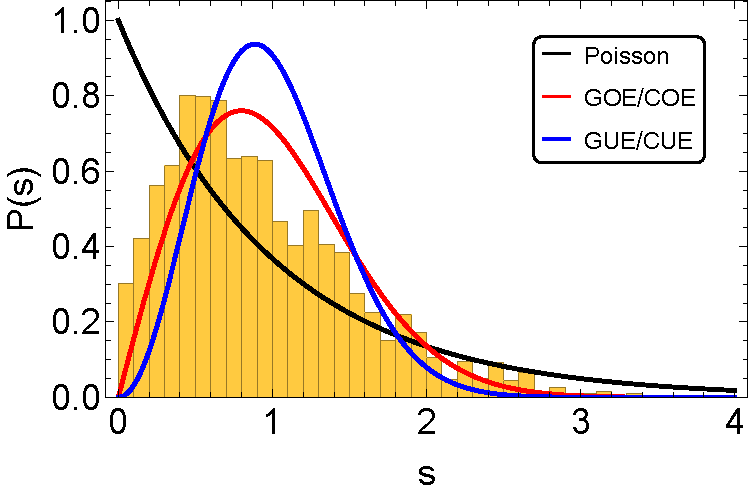
\includegraphics[width=0.8\textwidth]{SpacingCardQuditHaad.pdf}
    \caption{Espaciamiento a primer vecino de las eigenfases del operador evolución.}
\end{figure}
\begin{figure}[H]
    \centering
    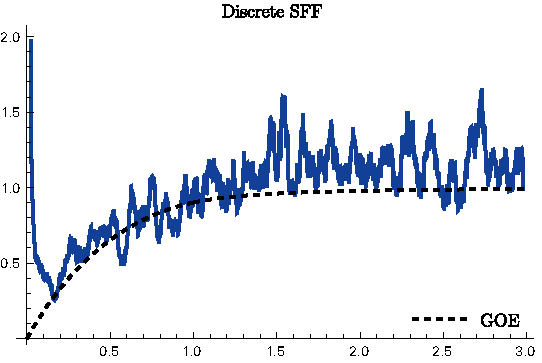
\includegraphics[width=0.8\textwidth]{SFFCardQuditHaad.pdf}
    \caption{Factor de forma espectral de las eigenfases del operador evolución.}
\end{figure}

\end{itemize}
\subsubsection{Monedad de Fourier}
Dada según
\begin{equation}
    F_4 = \frac{1}{2}
    \begin{pmatrix}
        1 &  1 &  1 &  1 \\
        1 &  i & -1 & -i \\
        1 & -1 &  1 & -1 \\
        1 & -i & -1 &  i
    \end{pmatrix}
\end{equation}
\begin{itemize}

\item \textbf{\large Para un estadio rectangular:}

Considerando un estadio rectangular, con dimensiones $L_x=35$ y $L_y=25$:
\begin{figure}[H]
    \centering
    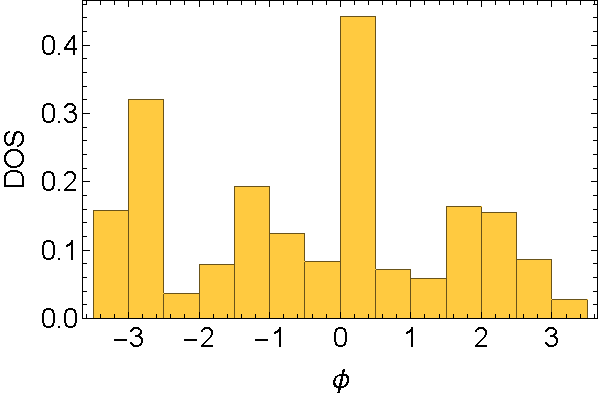
\includegraphics[width=0.8\textwidth]{DoSRectQuditFourier.pdf}
    \caption{DoS de las eigenfases del operador evolución.}
\end{figure}
Para esta moneda no fue necesario emplear un filtrado en las eigenfases.
\begin{figure}[H]
    \centering
    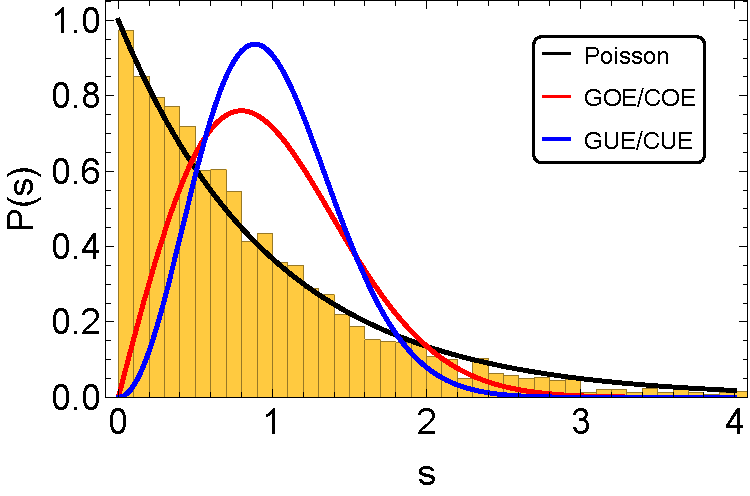
\includegraphics[width=0.8\textwidth]{SpacingRectQuditFourier.pdf}
    \caption{Espaciamiento a primer vecino de las eigenfases del operador evolución.}
\end{figure}
\begin{figure}[H]
    \centering
    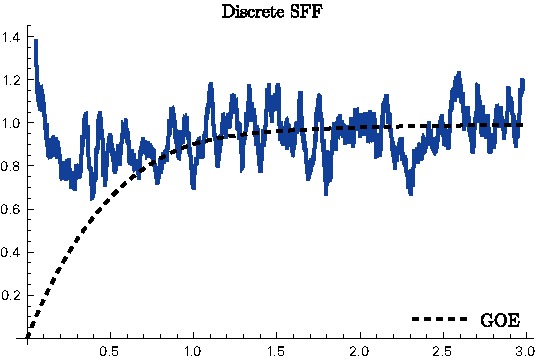
\includegraphics[width=0.8\textwidth]{SFFRectQuditFourier.pdf}
    \caption{Factor de forma espectral de las eigenfases del operador evolución.}
\end{figure}
\hfill
\item \textbf{\large Para un estadio bunimovich:}

 Empleando ahora un estadio bunimovich, de dimensiones $L=30$ y $R=25$.
\begin{figure}[H]
    \centering
    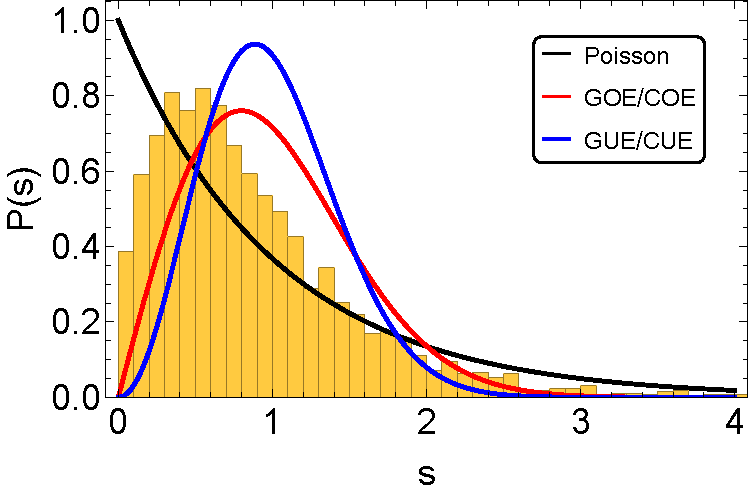
\includegraphics[width=0.8\textwidth]{SpacingBunQuditFourier.pdf}
    \caption{Espaciamiento a primer vecino de las eigenfases del operador evolución.}
\end{figure}
\begin{figure}[H]
    \centering
    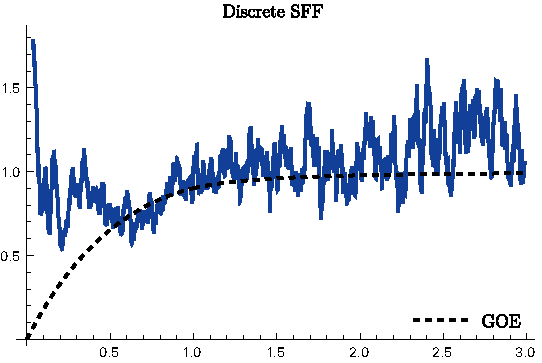
\includegraphics[width=0.8\textwidth]{SFFBunQuditFourier.pdf}
    \caption{Factor de forma espectral de las eigenfases del operador evolución.}
\end{figure}

\item \textbf{\large Para un estadio elipse:}

 Empleando ahora un estadio elipse, con semi-eje mayor de $A=20$ y semi-eje menor de $B=15$.
\begin{figure}[H]
    \centering
    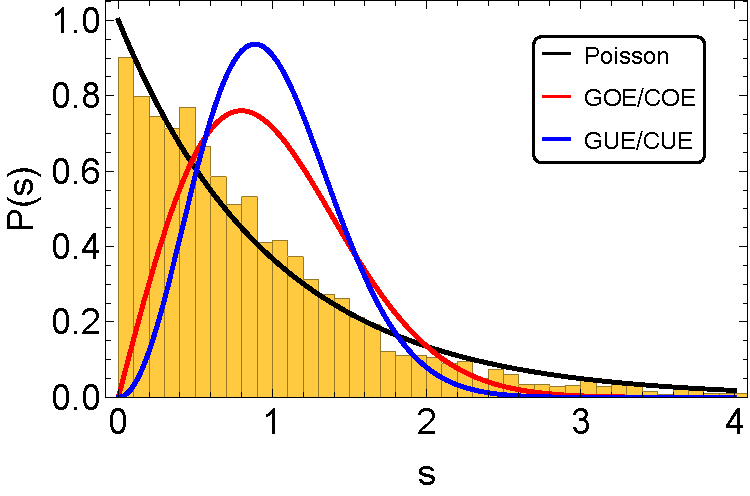
\includegraphics[width=0.8\textwidth]{SpacingElipseQuditFourier.pdf}
    \caption{Espaciamiento a primer vecino de las eigenfases del operador evolución.}
\end{figure}
\begin{figure}[H]
    \centering
    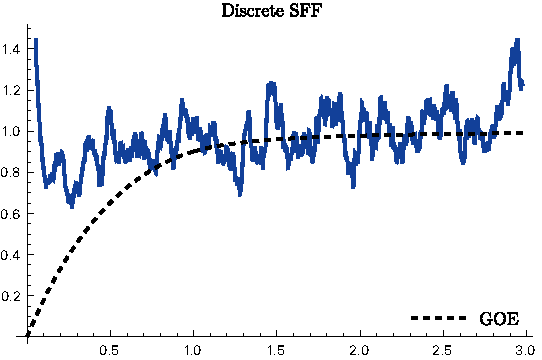
\includegraphics[width=0.8\textwidth]{SFFElipseQuditFourier.pdf}
    \caption{Factor de forma espectral de las eigenfases del operador evolución.}
\end{figure}

\item \textbf{\large Para un estadio cardioide:}

 Empleando ahora un estadio cardiode, con parámetro de escala $R=7$, siendo $r=2R(1-\cos(\theta))$
\begin{figure}[H]
    \centering
    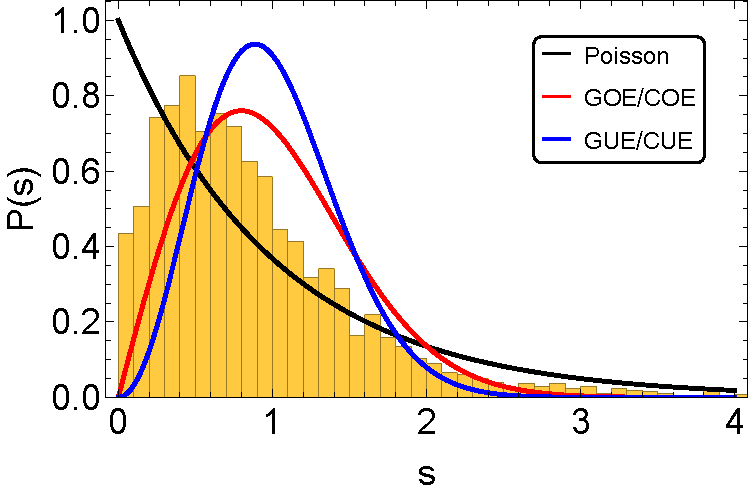
\includegraphics[width=0.8\textwidth]{SpacingCardQuditFourier.pdf}
    \caption{Espaciamiento a primer vecino de las eigenfases del operador evolución.}
\end{figure}
\begin{figure}[H]
    \centering
    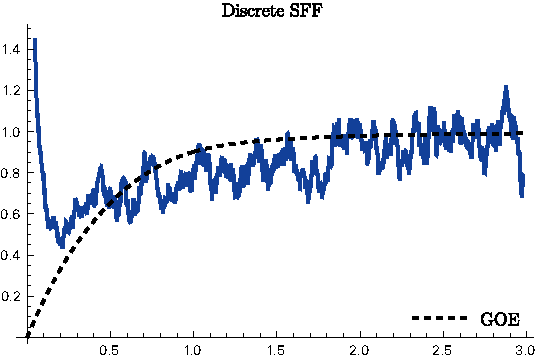
\includegraphics[width=0.8\textwidth]{SFFCardQuditFourier.pdf}
    \caption{Factor de forma espectral de las eigenfases del operador evolución.}
\end{figure}

\end{itemize}

\end{document}